\section{Columbia Game Corpus}

\begin{figure}
\centering
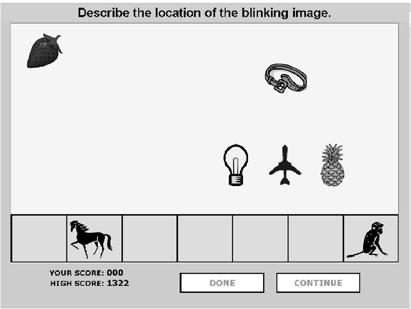
\includegraphics[width=10cm]{images/columbia_games.jpg}
\caption{Juego del Columbia Games}
\label{tablero_columbia_games}
\end{figure}

\newcommand{\cardgame} {\emph{Juego de cartas}}
\newcommand{\objectgame} {\emph{Juego de objetos}}

WTF REESCRIBIR ESTO NO TIENE SENTIDO

Nuestro corpus \ref{GRAV2009} consiste en doce conversaciones diádicas (i.e., con dos participantes) entre trece personas angloparlantes distintas. En cada sesión, se sentó a dos participantes (quienes no se conocían previamente) en una cabina profesional de grabación, cara a cara a ambos lados de una mesa, y con una cortina opaca colgando entre ellos para evitar la comunicación visual.


Las grabaciones se hicieron en 44 kHz, 16 bits con un canal separado para cada hablante; luego fueron guardadas en 16 kHz para el presente estudio. Cada sesión duró aproximadamente 45 minutos, totalizando 9 horas de diálogos, 70.259 palabras (2.037 únicas) para todo el cuerpo de datos.


Los participantes contaron con sendas computadoras portátiles conectadas entre sí, en las cuales jugaron una serie de juegos simples que requerían de comunicación verbal. Por ejemplo, en uno de tales juegos, ambas computadoras muestran un tablero con varios objetos \ref{tablero_columbia_games}, todos en la misma posición excepto por uno, el objetivo, que aparece en un lugar distinto en cada computadora.

\subsection{\cardgame}
\begin{figure}
\centering
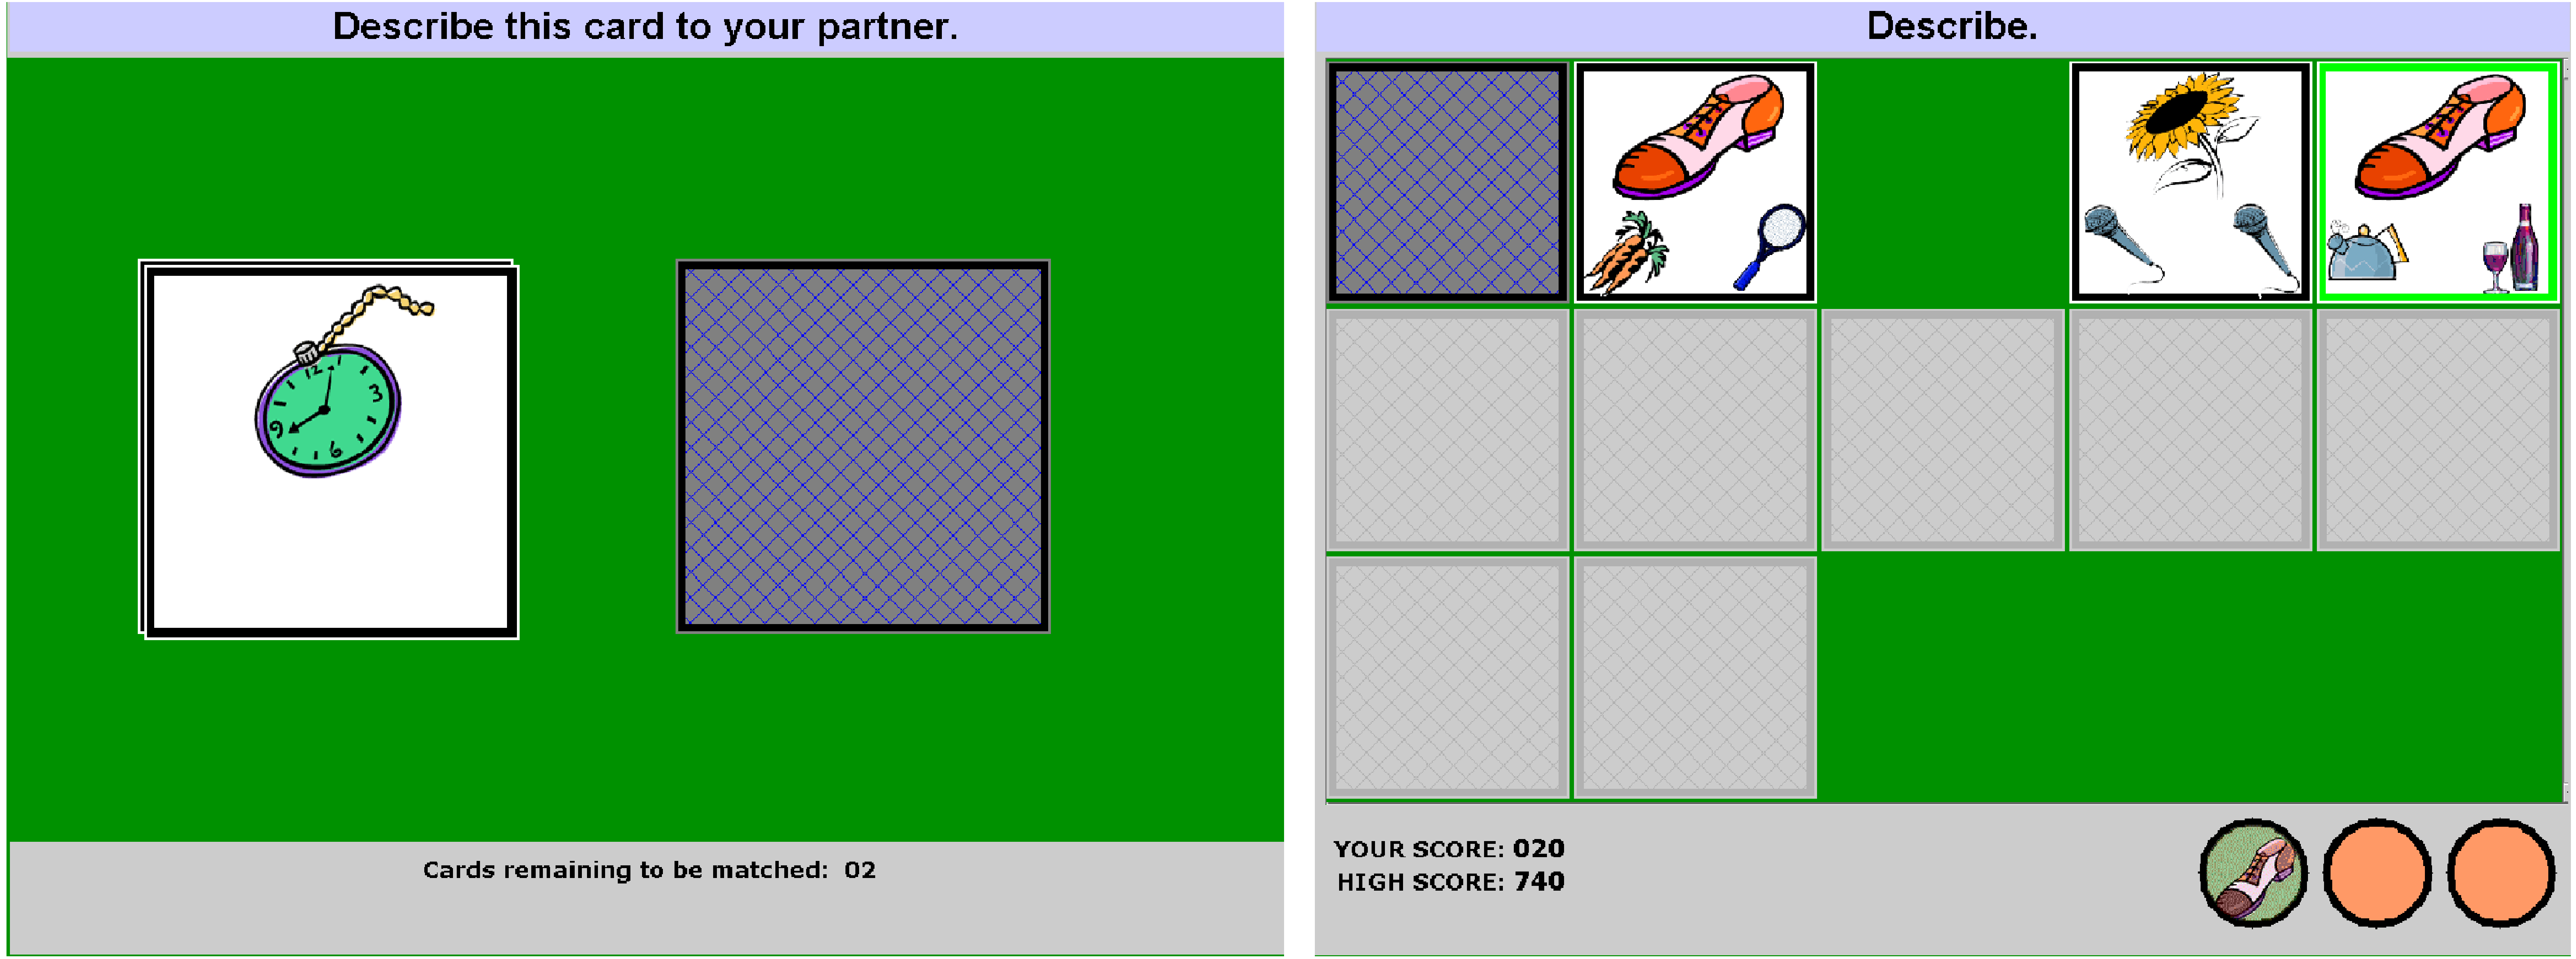
\includegraphics[width=10cm]{images/columbia_games_card_game.png}
\caption{Juego del Columbia Games - Juego de Cartas}
\label{tablero_columbia_games}
\end{figure}


En primer lugar, los sujetos del experimento jugaron tres instancias del \cardgame, donde cada una se subdividía en dos partes. En la etapa inicial del juego, la pantalla de cada jugador mostró un mazo de 9 o 10 cartas. A uno de los jugadores se le pidió que describa la carta en el tope del mazo, mientras que el otro debía buscar en su mazo para encontrar la carta en cuestión, apretando un botón al finalizar ésto. Ésto contínua hasta que las cartas del primer jugador se acaben.


En la segunda parte del \cardgame, cada jugador tenía una mesa con 12 cartas en ella, inicialmente boca abajo. Mientras el juego comienza, la primera carta de uno de los jugadores se dió vuelta. Este jugador (el Descriptor) debía describir dicha carta al otro jugador (el Buscador), cuya labor era buscar dicha carta en su mesa. Si el Buscador podía encontrar una carta que satisficiese la descripción dada, declararía un acierto y recibiría puntos proporcionales al acierto.

\subsection{\objectgame}


\subsection{Anotaciones sobre comportamiento social}

Varios aspectos del comportamiento de los jugadores durante los juegos de Objeto fueron anotados mediante la herramienta de crowdsourcing \emph{Mechanical Turk}. Cada anotador escuchó un clip de un juego y tuvo que responder a las siguientes preguntas (para cada uno de los sujetos):

\begin{itemize}
  \item ¿el sujeto le hace difícil hablar a su compañero?
  \item ¿el sujeto parece comprometido con el juego?
  \item ¿al sujeto no le agrada su compañero?
  \item ¿el sujeto dirige la conversación?
  \item ¿el sujeto contribuye para el éxito del equipo?
  \item ¿el sujeto alienta a su compañero?
  \item ¿el sujeto se expresa correctamente?
  \item ¿el sujeto intenta acaparar la conversación?
\end{itemize}

entre otras. Cada uno de estos clips fue puntuado por cinco anotadores, que respondieron por sí o por no. El puntaje que recibe cada una de las preguntas (a las cuales llamaremos a partir de ahora \emph{variables sociales}) consiste en la cantidad de respuestas afirmativas que recibió, teniendo un rango de 0 a 5.

